\documentclass[12pt]{acmart}
\usepackage[utf8]{inputenc}
\usepackage{myhandout}
\usepackage[options ]{algorithm2e}
\usepackage{tikz}
\usepackage{float}
\usepackage{amsmath}
\usepackage{enumitem}

\title{Reflections on CSC630 Spring 2020: Generalizations in Neural Network}
\author{Gurman Singh}
\email{gsingh23@ncsu.edu}

\begin{document}

\maketitle

\section{Introduction}
As a part of this independent study, we tried to understand the scopes and possibilities in the field of Artificial General Intelligence. We basically covered neural networks and convolution and tried to understand how we can implement generalizations in Neural Networks.

In this study, 
\begin{enumerate}
    \item We learnt about deep neural networks and their implementation using pytorch\cite{pytorch}.
    \item We learnt about how these networks work and concepts like gradient and back-propagation and how they help in bringing the idea of neural networks to reality\cite{backpropagation}.
    \item We learnt about the working of GPU's and how they are being utilized in implementation of Neural Networks in a faster manner using the Google Colab notebooks\cite{colab}.
    \item Finally, we explored and tried one of the ways we can bring in generalisations to the field of Artificial Intelligence using Neural Networks.
\end{enumerate}

The main challenge that we faced in this exploration was that how we can generalize Neural networks that are comparable to human like general intelligence.

We believe that neural networks are the closest we have been yet, towards a biological brain. So we continued on this and thought of how can we modify or build something that is more general than the concepts that we already have.

The main idea was that instead of having a single Neural network that could be trained to do a specific task, lets build an architecture of neural networks that could perform more generic tasks than the one's it is trained for.

\section{Background}
\subsection{Neural Network}
We started off by learning what neural networks (Figure \ref{fig:NN}) are\cite{backpropagation}\cite{NN}\cite{3b1b}, implementing a simple neural network that gave $98\%$ accuracy on MNIST database\cite{MNIST}(9783 out of 10000 test images identified correctly).
The network consisted of:
\begin{enumerate}
    \item Input of $28$$\times$$28$ gray-scale images of handwritten digits.
    \item Two hidden layers of $200$ nodes each.
    \item An output layer of $10$ nodes to identify the digit on the image.
\end{enumerate}
\begin{figure}[H]
  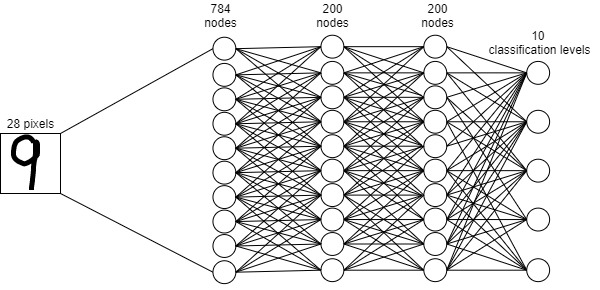
\includegraphics[width=\linewidth]{NN.jpg}
  \caption{Fully connected Neural Network design, given a handwritten input of $9$}
  \label{fig:NN}
\end{figure}


\subsection{Convolutional Neural Network}
Convolution specifically helps take a different stance towards the input. In a fully connected network, the 2-D input is converted into a single dimensional array and fed to the network, whereas in convolution, the relative positioning of the nodes in 2 dimensions is also taken into consideration, i.e., the nodes that are closer together in 2 dimensional input get to keep there positioning when fed into the convolutional network \cite{CNN}.

In convolution, the input channels are sent to a set of filters. The filters are usually smaller than the input channels size. These filters move over the input to create a output channels. After some layers of convolution, the output is fed into the fully connected network.

But since the simple Neural network already gave us $98\%$ accuracy, we had to find some other way to realise the power of convolution. We used data augmentation to challenge up things for our network.

\begin{figure}[H]
  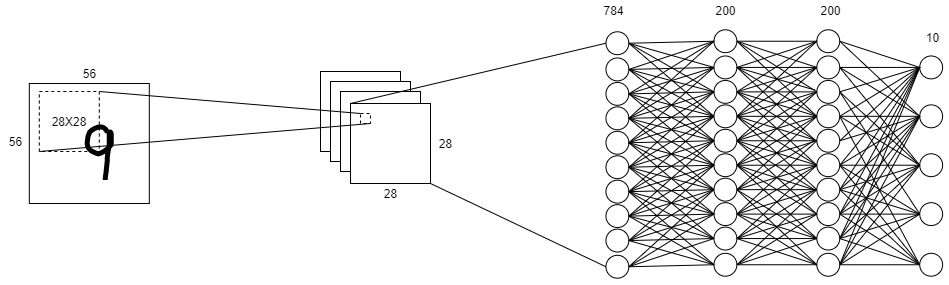
\includegraphics[width=\linewidth]{Convolution.jpg}
  \caption{Basic Convolution architecture.}
  \label{fig:Convolution}
\end{figure}


\section{Technical Approach}
\subsection{Data Augmentation}
We augmented the input data by converting the $28$$\times$$28$ input to $56$$\times$$56$ size input as shown in Figure \ref{fig:Convolution}. We took the original image and imposed it on top of a $56$$\times$$56$ array of all zeroes. The position of the smaller image could be randomly anywhere over the bigger image, but it was made sure that the smaller image is always fully contained inside the bigger one (Figure: \ref{fig:Shuffle}).

For starters, we only placed the smaller image on one of the four quadrants of the larger image, in order to test that if we train the network on one of the quadrants, will it be able to identify the digits on other quadrants.

\begin{figure}[H]
  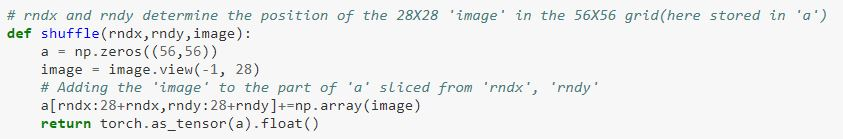
\includegraphics[width=\linewidth]{Shuffle.JPG}
  \caption{Data augmentation snippet.}
  \label{fig:Shuffle}
\end{figure}


\subsection{Search for Symmetry}
After training the network mentioned above, we tested images which were not in one of the quadrants, the results had the following pattern in them:

The results were poorest when tested in the center and the accuracy increased as the smaller image moved to the edges of the larger image and approached from $14\%$ at the center to $96\%$ accuracy as the image approached the corners during the tests.

This symmetrical result was obtained by placing the smaller image over one of the quadrants during training.

\subsection{Uniform Accuracy}
Later on, when training set had the smaller image placed anywhere on the larger image independent of the quadrant, uniform results of $95\%$ accuracy were achieved at all locations of the $56$$\times$$56$ image.

% After some hyper parameter searching, it was able to identify the $28$$\times$$28$ digits in the $56$$\times$$56$ image $94\%$ of the times from a set of 10,000 images.
These above results (both symmetric and uniform) were obtained only after intensive hyper-parameter search.

The most important parameter having the greatest impact came out to be the size of the filter at the first convolution layer, we got the best results when the size of the filter was equal to the size of the smaller image, i.e., $28$$\times$$28$.
The intuition behind keeping this size was that the network(or the first convolution layer) should be able to identify the digits from the $56$$\times$$56$ image.

\subsection{The Layered Network(Idea)}
The idea is to have a structure of networks, in which each network is assigned to do a specific task and different networks work with each other and use inputs and outputs from each other to reach complex conclusions.
In our particular case, we shall have 2 networks as shown in Figure \ref{fig:Layered Convolution}):
\begin{figure}[H]
  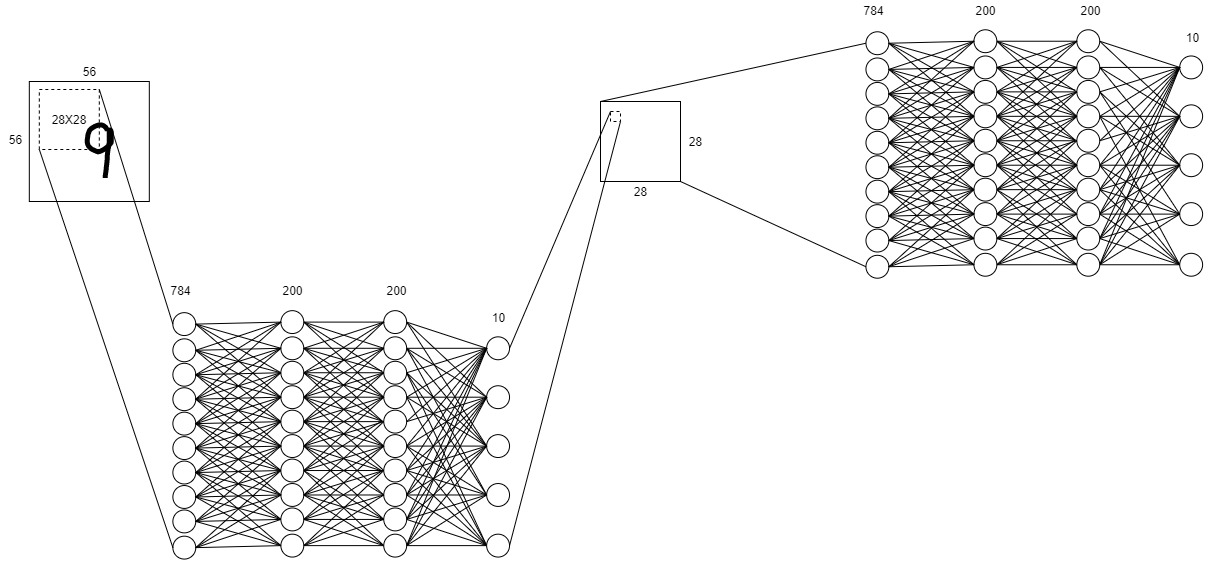
\includegraphics[width=\linewidth]{Layered-Convolution.jpg}
  \caption{Layered Neural Network architecture.}
  \label{fig:Layered Convolution}
\end{figure}
\begin{figure}[H]
  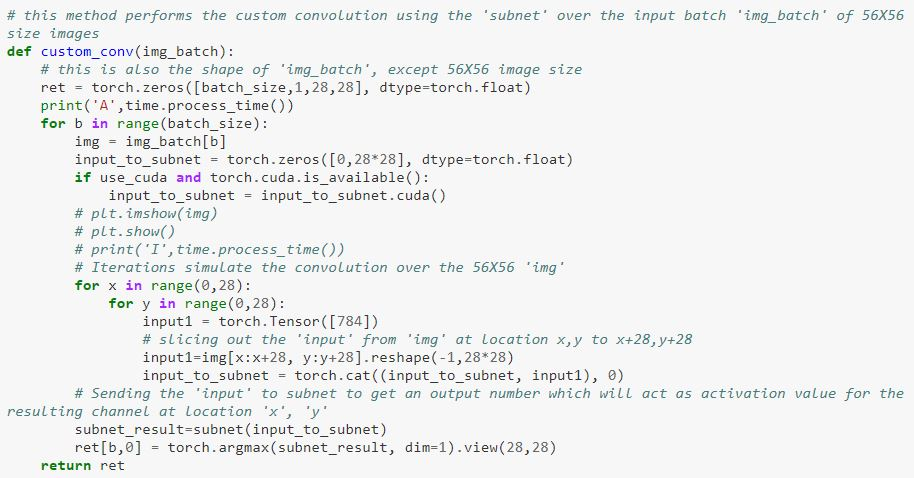
\includegraphics[width=\linewidth]{Custom_Conv.JPG}
  \caption{Manual Convolution performed on the input image batch.}
  \label{fig:Custom_Conv}
\end{figure}

\begin{enumerate}
    \item The first network will be a simple fully connected neural network as made in the beginning of this course which is trained to identify the $28$$\times$$28$ digits. It will simply take the $28$$\times$$28$ image as input and output what digit the image represents.
    \item The second network will be trained to utilize the capabilities of the first network to improve the accuracy of $56$$\times$$56$ size images. The plan is that the first filter of convolution will be mapped with the input of the first network. Once that is done, and the first filter travels over the image, every new position of the filter is sent as an input to the first network which in turn gives out an output, this whole process will give us a new channel which is the result of convolution of our $56$$\times$$56$ image with the first network, this output will further travel down the network including convolution and fully connected network as shown in Figure \ref{fig:Custom_Conv}.
\end{enumerate}

We shall evaluate our results by testing the trained network over a set of $56$$\times$$56$ images that contain handwritten digits of size $28$$\times$$28$ placed randomly anywhere over the larger image. The final accuracy will be a percentage of images recognized correctly by the network out of the whole data set.



Once this whole network is trained, it is expected to give out even more generic results, and can be used to identify digits on an image of any size. Or we can use multiple networks at layer 1, each of who would be trained to learn/identify something specific.

\section{Results}
\subsection{Training Details}

Following are the final network details,

\begin{table}[H]
    % \caption{table label}
    \begin{tabular}{|l|l|l|}
    \hline
    Parameter           & Value\\ \hline
    Training data set   & $60,000$ augmented images \\ \hline
    Testing data set    & $10,000$ augmented images \\ \hline
    Batch size          & $200$                     \\ \hline
    Number of epochs    & $10$                      \\ \hline
    Learning rate       & $0.01$                    \\ \hline
    Momentum            & $0.9$                     \\ \hline
    \end{tabular}
\end{table}

% \begin{itemize}
%     \item A training data set of $60,000$ augmented images
%     \item A testing data set of $10,000$ augmented images
%     \item A batch size of $200$
%     \item $10$ epochs
%     \item learning rate of $0.01$
%     \item momentum of $0.9$
% \end{itemize}

\subsection{Accuracy}
The final accuracy achieved was $95\%$.

The aim of this study was not to achieve high accuracy but to achieve generalization, as discussed in the next section (\nameref{Future Direction}).

\section{Discussion}
\subsection{Performance Challenges}
The current network takes approximately $45$ minutes to train, because of the manual convolution that we perform. This time was brought down to $45$ from more than $5$ hours of training time by manipulations in bulk data handling after a better understanding of GPU processing and pytorch library.
We believe the performance can further be improved by processing even more data in parallel and by more investment into the programming of the network.

\subsection{Future Direction}
\label{Future Direction}
The current study did not prove that generalization is possible by way of a composition of neural networks, but it proves that this way is possible if chosen to be explored further.

The few ways in which generalization can be achieved are as follows:
\begin{itemize}
    \item Specialized networks
    
    This architecture utilizes multiple small networks each of which would be specialized to perform a specific task and there would be a higher level network that would be trained to read and understand the outputs of these smaller networks give out relevant output.
    \item The Confusion/Confidence Factor
    
    If we want to achieve generalization, it is very important to have a concept of confusion or confidence in a network's output. i.e., The network should be able to tell how confident another network is while trying to read its output and whether to trust other network's output or not.
    
    This can be achieved in our case if the smaller networks give out more details about their output(like reasoning), rather than just a yes/no answer.
    
    We could not test this because the memory requirements of training such a network were more than the available memory resources.

\section{Conclusion}
In summary, we learnt from scratch what neural networks are, how powerful they can be, how to implement them. And then we explored them to learn more about their relevance with the biological brain. Finally we proposed and built a network that could be a possible simulation of how the human mind recognizes different categories of the world model.

Their is still much more work to be done and explored in this area, the most challenging and important one being the implementation of confusion in neural networks.

\end{itemize}


\begin{thebibliography}{}
    \bibitem{backpropagation}
    Rumelhart, D., Hinton, G. & Williams, R. Learning representations by back-propagating errors. Nature 323, 533–536 (1986). https://doi.org/10.1038/323533a0

    \bibitem{MNIST}
    \textit{http://yann.lecun.com/exdb/mnist/}

    
    \bibitem{pytorch}
    \textit{https://pytorch.org/}

    \bibitem{colab}
    \textit{https://colab.research.google.com/}

    \bibitem{3b1b}
    \textit{https://www.youtube.com/watch?v=aircAruvnKk&list=PLZHQObOWTQDNU6R1\_67000Dx\_ZCJB-3pi}
    
    \bibitem{NN}
    \textit{https://adventuresinmachinelearning.com/pytorch-tutorial-deep-learning/}
    
    \bibitem{CNN}
    \textit{https://adventuresinmachinelearning.com/convolutional-neural-networks-tutorial-in-pytorch/}

\end{thebibliography}

\end{document}
